\documentclass{standalone}
\usepackage{tikz}
\usetikzlibrary{patterns, positioning}
\usepackage[sfdefault]{ClearSans} %% option 'sfdefault' activates Clear Sans as the default text font
\usepackage[T1]{fontenc}

\begin{document}
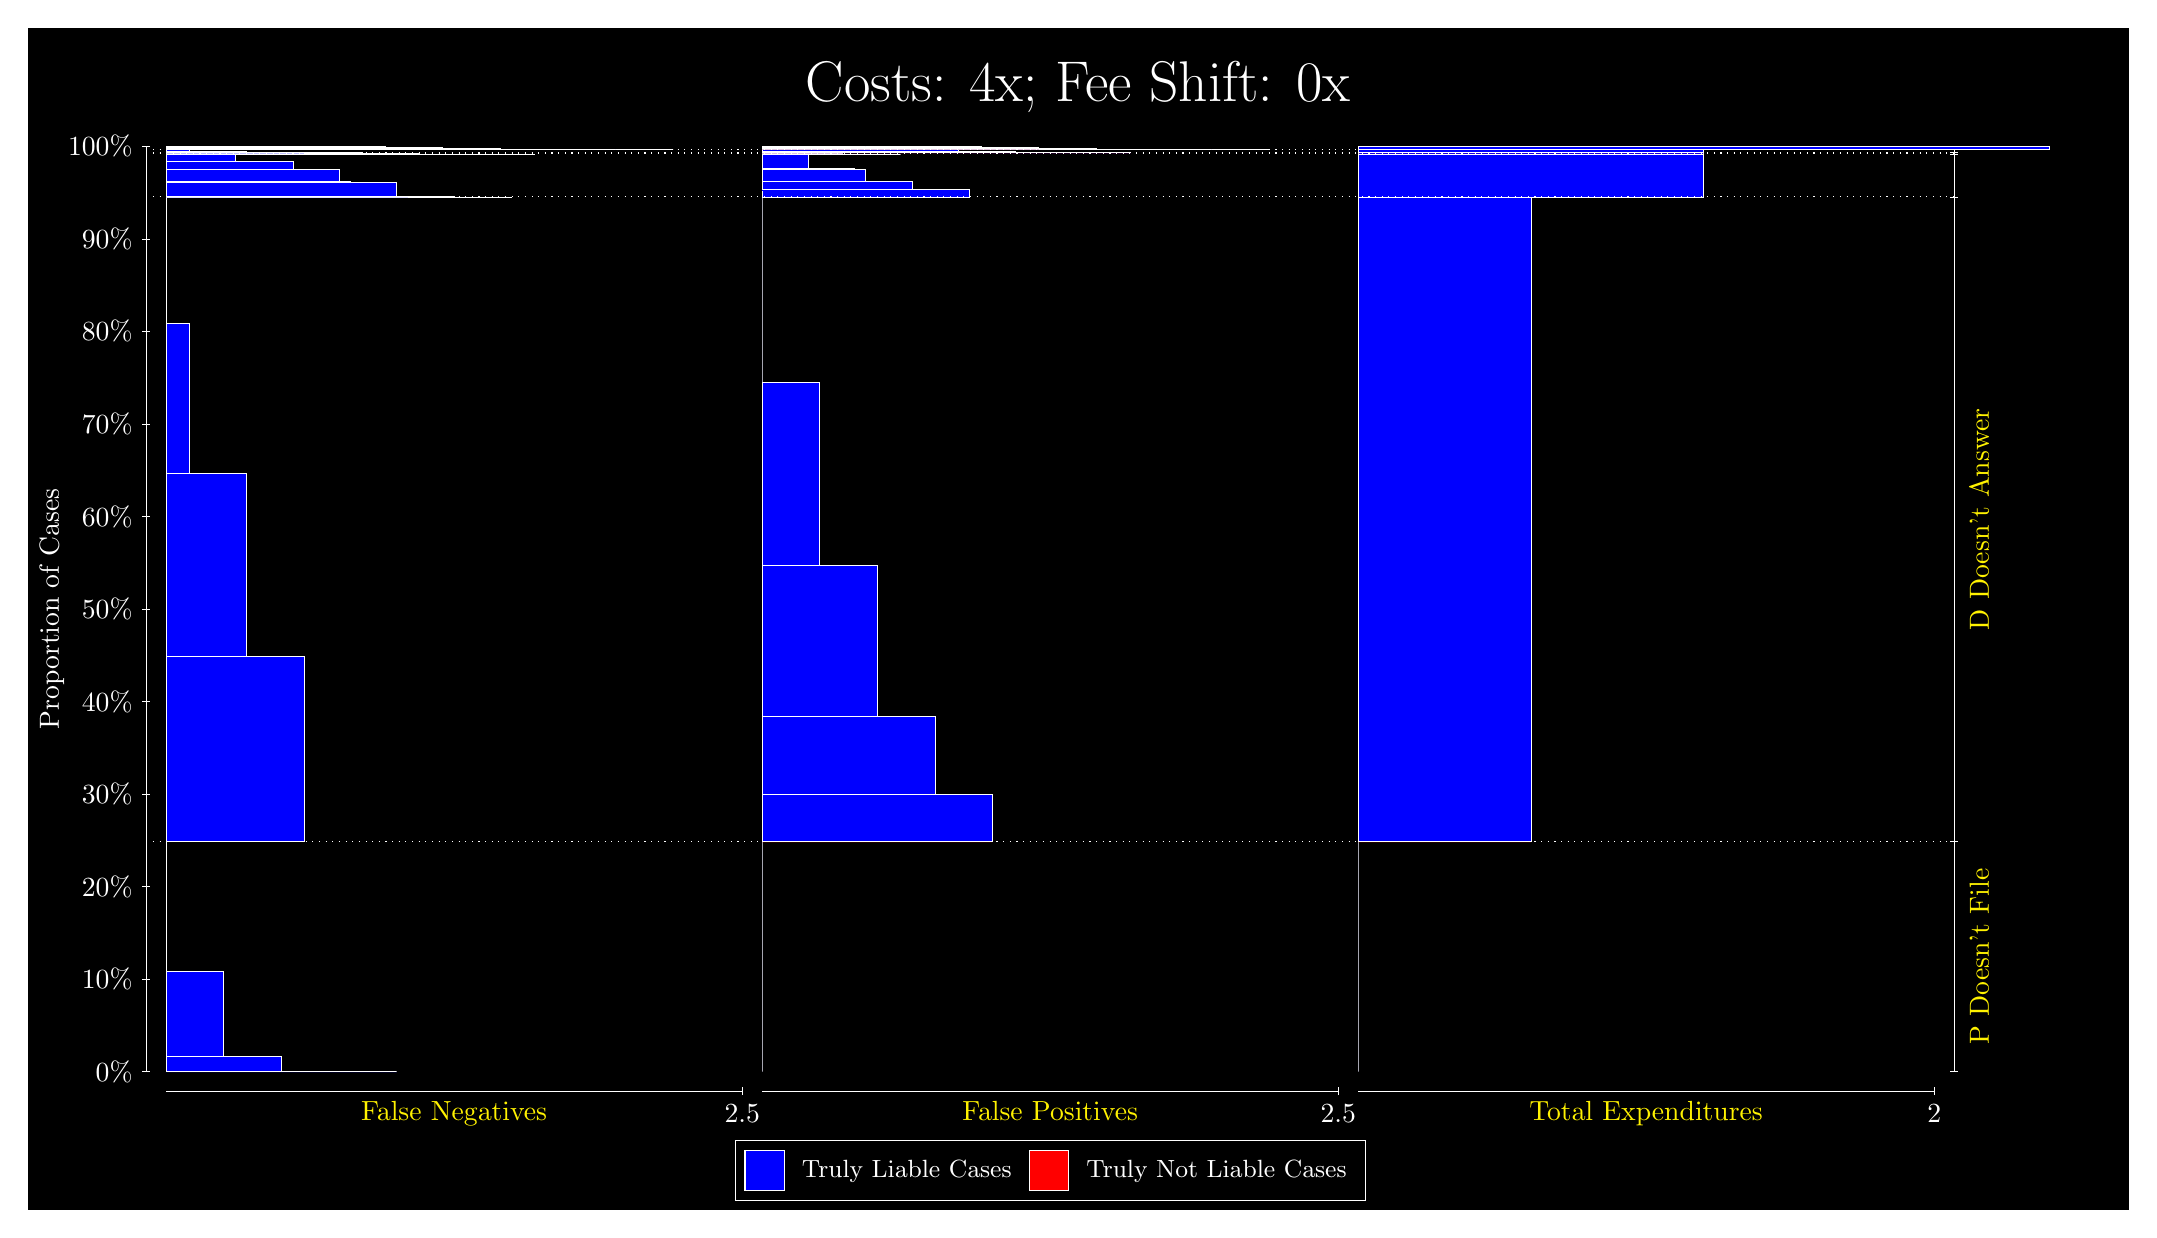
\begin{tikzpicture}
\draw[fill=black] (0,0) rectangle (26.667,15);
\draw[text=white] (0,13.5) rectangle (26.667,15) node[midway] {\huge Costs: 4x; Fee Shift: 0x};
\draw[white, very thin] (1.5,1.75) -- (1.5,13.5);
\node[rotate=90, text=white, anchor=center] at (0.3, 7.625) {Proportion of Cases};
\draw[white, very thin] (1.45,1.75) -- (1.55,1.75);
\node[text=white, anchor=east] at (1.45, 1.75) {0\%};
\draw[white, very thin] (1.45,2.925) -- (1.55,2.925);
\node[text=white, anchor=east] at (1.45, 2.925) {10\%};
\draw[white, very thin] (1.45,4.1) -- (1.55,4.1);
\node[text=white, anchor=east] at (1.45, 4.1) {20\%};
\draw[white, very thin] (1.45,5.275) -- (1.55,5.275);
\node[text=white, anchor=east] at (1.45, 5.275) {30\%};
\draw[white, very thin] (1.45,6.45) -- (1.55,6.45);
\node[text=white, anchor=east] at (1.45, 6.45) {40\%};
\draw[white, very thin] (1.45,7.625) -- (1.55,7.625);
\node[text=white, anchor=east] at (1.45, 7.625) {50\%};
\draw[white, very thin] (1.45,8.8) -- (1.55,8.8);
\node[text=white, anchor=east] at (1.45, 8.8) {60\%};
\draw[white, very thin] (1.45,9.975) -- (1.55,9.975);
\node[text=white, anchor=east] at (1.45, 9.975) {70\%};
\draw[white, very thin] (1.45,11.15) -- (1.55,11.15);
\node[text=white, anchor=east] at (1.45, 11.15) {80\%};
\draw[white, very thin] (1.45,12.325) -- (1.55,12.325);
\node[text=white, anchor=east] at (1.45, 12.325) {90\%};
\draw[white, very thin] (1.45,13.5) -- (1.55,13.5);
\node[text=white, anchor=east] at (1.45, 13.5) {100\%};

\draw[white, very thin] (24.457,1.75) -- (24.457,13.5);
\draw[white, very thin] (24.407,1.75) -- (24.507,1.75);
\node[anchor=west] at (24.407, 1.75) {};
\draw[white, very thin] (24.407,4.6695) -- (24.507,4.6695);
\node[anchor=west] at (24.407, 4.6695) {};
\draw[white, very thin] (24.407,12.858) -- (24.507,12.858);
\node[anchor=west] at (24.407, 12.858) {};
\draw[white, very thin] (24.407,13.405) -- (24.507,13.405);
\node[anchor=west] at (24.407, 13.405) {};
\draw[white, very thin] (24.407,13.419) -- (24.507,13.419);
\node[anchor=west] at (24.407, 13.419) {};
\draw[white, very thin] (24.407,13.461) -- (24.507,13.461);
\node[anchor=west] at (24.407, 13.461) {};
\draw[white, very thin] (24.407,13.5) -- (24.507,13.5);
\node[anchor=west] at (24.407, 13.5) {};

\draw[white, very thin, fill=blue] (1.75,1.75) rectangle (4.6775,1.75);
\draw[white, very thin, fill=blue] (1.75,1.75) rectangle (3.9457,1.7516);
\draw[white, very thin, fill=blue] (1.75,1.7516) rectangle (3.2138,1.9388);
\draw[white, very thin, fill=blue] (1.75,1.9388) rectangle (2.4819,3.0197);
\draw[white, very thin, fill=red] (1.75,3.0197) rectangle (1.75,3.0197);
\draw[white, very thin, fill=blue] (1.75,3.0197) rectangle (1.75,4.6695);
\draw[white, very thin, fill=blue] (1.75,4.6695) rectangle (3.5065,7.0192);
\draw[white, very thin, fill=blue] (1.75,7.0192) rectangle (2.7746,9.3442);
\draw[white, very thin, fill=blue] (1.75,9.3442) rectangle (2.0428,11.259);
\draw[white, very thin, fill=red] (1.75,11.259) rectangle (1.75,11.259);
\draw[white, very thin, fill=blue] (1.75,11.259) rectangle (1.75,12.858);
\draw[white, very thin, fill=blue] (1.75,12.858) rectangle (6.1413,12.858);
\draw[white, very thin, fill=blue] (1.75,12.858) rectangle (5.5558,12.858);
\draw[white, very thin, fill=blue] (1.75,12.858) rectangle (5.4094,12.861);
\draw[white, very thin, fill=blue] (1.75,12.861) rectangle (4.8239,12.861);
\draw[white, very thin, fill=blue] (1.75,12.861) rectangle (4.6775,13.044);
\draw[white, very thin, fill=blue] (1.75,13.044) rectangle (4.092,13.051);
\draw[white, very thin, fill=blue] (1.75,13.051) rectangle (3.9457,13.203);
\draw[white, very thin, fill=blue] (1.75,13.203) rectangle (3.3602,13.311);
\draw[white, very thin, fill=blue] (1.75,13.311) rectangle (3.2138,13.313);
\draw[white, very thin, fill=blue] (1.75,13.313) rectangle (2.6283,13.405);
\draw[white, very thin, fill=red] (1.75,13.405) rectangle (1.75,13.405);
\draw[white, very thin, fill=blue] (1.75,13.405) rectangle (6.4341,13.405);
\draw[white, very thin, fill=blue] (1.75,13.405) rectangle (5.7022,13.405);
\draw[white, very thin, fill=blue] (1.75,13.405) rectangle (4.9703,13.412);
\draw[white, very thin, fill=blue] (1.75,13.412) rectangle (4.2384,13.419);
\draw[white, very thin, fill=blue] (1.75,13.419) rectangle (3.5065,13.419);
\draw[white, very thin, fill=red] (1.75,13.419) rectangle (1.75,13.419);
\draw[white, very thin, fill=blue] (1.75,13.419) rectangle (3.5065,13.419);
\draw[white, very thin, fill=blue] (1.75,13.419) rectangle (2.7746,13.438);
\draw[white, very thin, fill=blue] (1.75,13.438) rectangle (2.0428,13.458);
\draw[white, very thin, fill=red] (1.75,13.458) rectangle (1.75,13.458);
\draw[white, very thin, fill=blue] (1.75,13.458) rectangle (1.75,13.461);
\draw[white, very thin, fill=blue] (1.75,13.461) rectangle (8.1906,13.461);
\draw[white, very thin, fill=blue] (1.75,13.461) rectangle (7.4587,13.461);
\draw[white, very thin, fill=blue] (1.75,13.461) rectangle (6.7268,13.462);
\draw[white, very thin, fill=blue] (1.75,13.462) rectangle (5.9949,13.471);
\draw[white, very thin, fill=blue] (1.75,13.471) rectangle (5.2631,13.49);
\draw[white, very thin, fill=blue] (1.75,13.49) rectangle (4.5312,13.499);
\draw[white, very thin, fill=blue] (1.75,13.499) rectangle (3.7993,13.5);
\draw[white, very thin, fill=blue] (1.75,13.5) rectangle (3.0674,13.5);
\draw[white, very thin, fill=blue] (1.75,13.5) rectangle (2.3355,13.5);
\draw[white, very thin, fill=red] (1.75,13.5) rectangle (1.75,13.5);
\draw[white, very thin, fill=red] (9.3189,1.75) rectangle (9.3189,1.75);
\draw[white, very thin, fill=blue] (9.3189,1.75) rectangle (9.3189,4.6695);
\draw[white, very thin, fill=red] (9.3189,4.6695) rectangle (12.246,4.6695);
\draw[white, very thin, fill=blue] (9.3189,4.6695) rectangle (12.246,5.2755);
\draw[white, very thin, fill=blue] (9.3189,5.2755) rectangle (11.515,6.2676);
\draw[white, very thin, fill=blue] (9.3189,6.2676) rectangle (10.783,8.1828);
\draw[white, very thin, fill=blue] (9.3189,8.1828) rectangle (10.051,10.508);
\draw[white, very thin, fill=blue] (9.3189,10.508) rectangle (9.3189,12.858);
\draw[white, very thin, fill=red] (9.3189,12.858) rectangle (11.954,12.858);
\draw[white, very thin, fill=blue] (9.3189,12.858) rectangle (11.954,12.949);
\draw[white, very thin, fill=red] (9.3189,12.949) rectangle (11.368,12.949);
\draw[white, very thin, fill=blue] (9.3189,12.949) rectangle (11.368,12.951);
\draw[white, very thin, fill=blue] (9.3189,12.951) rectangle (11.222,13.059);
\draw[white, very thin, fill=blue] (9.3189,13.059) rectangle (10.636,13.211);
\draw[white, very thin, fill=blue] (9.3189,13.211) rectangle (10.49,13.218);
\draw[white, very thin, fill=blue] (9.3189,13.218) rectangle (9.9044,13.401);
\draw[white, very thin, fill=blue] (9.3189,13.401) rectangle (9.758,13.401);
\draw[white, very thin, fill=blue] (9.3189,13.401) rectangle (9.3189,13.405);
\draw[white, very thin, fill=red] (9.3189,13.405) rectangle (11.075,13.405);
\draw[white, very thin, fill=blue] (9.3189,13.405) rectangle (11.075,13.405);
\draw[white, very thin, fill=blue] (9.3189,13.405) rectangle (10.344,13.412);
\draw[white, very thin, fill=blue] (9.3189,13.412) rectangle (9.6116,13.419);
\draw[white, very thin, fill=blue] (9.3189,13.419) rectangle (9.3189,13.419);
\draw[white, very thin, fill=red] (9.3189,13.419) rectangle (14.003,13.419);
\draw[white, very thin, fill=blue] (9.3189,13.419) rectangle (14.003,13.419);
\draw[white, very thin, fill=blue] (9.3189,13.419) rectangle (13.271,13.422);
\draw[white, very thin, fill=blue] (9.3189,13.422) rectangle (12.539,13.443);
\draw[white, very thin, fill=blue] (9.3189,13.443) rectangle (11.807,13.461);
\draw[white, very thin, fill=blue] (9.3189,13.461) rectangle (11.075,13.461);
\draw[white, very thin, fill=red] (9.3189,13.461) rectangle (15.759,13.461);
\draw[white, very thin, fill=blue] (9.3189,13.461) rectangle (15.759,13.461);
\draw[white, very thin, fill=blue] (9.3189,13.461) rectangle (15.028,13.461);
\draw[white, very thin, fill=red] (9.3189,13.461) rectangle (15.028,13.461);
\draw[white, very thin, fill=blue] (9.3189,13.461) rectangle (15.028,13.461);
\draw[white, very thin, fill=blue] (9.3189,13.461) rectangle (14.296,13.462);
\draw[white, very thin, fill=red] (9.3189,13.462) rectangle (14.296,13.462);
\draw[white, very thin, fill=blue] (9.3189,13.462) rectangle (14.296,13.462);
\draw[white, very thin, fill=blue] (9.3189,13.462) rectangle (13.564,13.463);
\draw[white, very thin, fill=red] (9.3189,13.463) rectangle (13.564,13.463);
\draw[white, very thin, fill=blue] (9.3189,13.463) rectangle (13.564,13.471);
\draw[white, very thin, fill=blue] (9.3189,13.471) rectangle (12.832,13.471);
\draw[white, very thin, fill=red] (9.3189,13.471) rectangle (12.832,13.471);
\draw[white, very thin, fill=blue] (9.3189,13.471) rectangle (12.832,13.49);
\draw[white, very thin, fill=blue] (9.3189,13.49) rectangle (12.1,13.499);
\draw[white, very thin, fill=blue] (9.3189,13.499) rectangle (11.368,13.5);
\draw[white, very thin, fill=blue] (9.3189,13.5) rectangle (10.636,13.5);
\draw[white, very thin, fill=blue] (9.3189,13.5) rectangle (9.9044,13.5);
\draw[white, very thin, fill=red] (16.888,1.75) rectangle (16.888,1.75);
\draw[white, very thin, fill=blue] (16.888,1.75) rectangle (16.888,4.6695);
\draw[white, very thin, fill=red] (16.888,4.6695) rectangle (19.083,4.6695);
\draw[white, very thin, fill=blue] (16.888,4.6695) rectangle (19.083,12.858);
\draw[white, very thin, fill=red] (16.888,12.858) rectangle (21.279,12.858);
\draw[white, very thin, fill=blue] (16.888,12.858) rectangle (21.279,13.405);
\draw[white, very thin, fill=red] (16.888,13.405) rectangle (21.279,13.405);
\draw[white, very thin, fill=blue] (16.888,13.405) rectangle (21.279,13.419);
\draw[white, very thin, fill=red] (16.888,13.419) rectangle (21.279,13.419);
\draw[white, very thin, fill=blue] (16.888,13.419) rectangle (21.279,13.461);
\draw[white, very thin, fill=red] (16.888,13.461) rectangle (25.67,13.461);
\draw[white, very thin, fill=blue] (16.888,13.461) rectangle (25.67,13.462);
\draw[white, very thin, fill=red] (16.888,13.462) rectangle (25.67,13.462);
\draw[white, very thin, fill=blue] (16.888,13.462) rectangle (25.67,13.5);
\draw[white, dotted] (1.5,4.6695) -- (24.457,4.6695);
\draw[white, dotted] (1.5,12.858) -- (24.457,12.858);
\draw[white, dotted] (1.5,13.405) -- (24.457,13.405);
\draw[white, dotted] (1.5,13.419) -- (24.457,13.419);
\draw[white, dotted] (1.5,13.461) -- (24.457,13.461);
\draw[white, very thin] (1.75,1.5) -- (9.0689,1.5);
\node[text=yellow, anchor=north] at (5.4094, 1.5) {False Negatives};
\draw[white, very thin] (9.0689,1.45) -- (9.0689,1.55);
\node[text=white, anchor=north] at (9.0689, 1.45) {2.5};

\draw[white, very thin] (9.3189,1.5) -- (16.638,1.5);
\node[text=yellow, anchor=north] at (12.978, 1.5) {False Positives};
\draw[white, very thin] (16.638,1.45) -- (16.638,1.55);
\node[text=white, anchor=north] at (16.638, 1.45) {2.5};

\draw[white, very thin] (16.888,1.5) -- (24.207,1.5);
\node[text=yellow, anchor=north] at (20.547, 1.5) {Total Expenditures};
\draw[white, very thin] (24.207,1.45) -- (24.207,1.55);
\node[text=white, anchor=north] at (24.207, 1.45) {2};

\node[text=yellow, centered, rotate=90] at (24.777, 3.2098) {P Doesn't File};
\node[text=yellow, centered, rotate=90] at (24.777, 8.7635) {D Doesn't Answer};





\draw (12.978300999999998,1.5) node[draw=none] (baseCoordinate) {};
\begin{scope}[align=center]
        \matrix[scale=0.5, draw=white, below=0.5cm of baseCoordinate, nodes={draw}, column sep=0.1cm]{
            \node[rectangle, draw, minimum width=0.5cm, minimum height=0.5cm, fill=blue] {}; &
            \node[draw=none, font=\small, text=white] (B) {Truly Liable Cases}; &
            \node[rectangle, draw, minimum width=0.5cm, minimum height=0.5cm, fill=red] {}; &
            \node[draw=none, font=\small, text=white] (B) {Truly Not Liable Cases}; \\
            };
\end{scope}

\end{tikzpicture}
\end{document}